\documentclass[prc]{revtex4} \usepackage[dvips]{graphicx}
\usepackage{mathrsfs} \usepackage{amsfonts} \usepackage{lscape}

\usepackage{epic,eepic} \usepackage{amsmath} \usepackage{amssymb}
\usepackage[dvips]{epsfig} \usepackage[T1]{fontenc}
\usepackage{hyperref} \usepackage{bezier} \usepackage{pstricks}
\usepackage{dcolumn}% Align table columns on decimal point
\usepackage{bm}% bold math
%\usepackage{braket}
\usepackage[dvips]{graphicx} \usepackage{pst-plot}

\newcommand{\One}{\hat{\mathbf{1}}} \newcommand{\eff}{\text{eff}}
\newcommand{\Heff}{\hat{H}_\text{eff}}
\newcommand{\Veff}{\hat{V}_\text{eff}}
\newcommand{\braket}[1]{\langle#1\rangle}
\newcommand{\Span}{\operatorname{sp}}
\newcommand{\tr}{\operatorname{trace}}
\newcommand{\diag}{\operatorname{diag}}
\newcommand{\bra}[1]{\left\langle #1 \right|}
\newcommand{\ket}[1]{\left| #1 \right\rangle} \newcommand{\element}[3]
           {\bra{#1}#2\ket{#3}}

\newcommand{\normord}[1]{ \left\{#1\right\} }

\usepackage{amsmath}
%\newcommand{\be}{\begin{equation}}
%\newcommand{\ee}{\end{equation}}
%\newcommand{\OP}[1]{{\bf\widehat{#1}}}

\begin{document}

\begin{center}
{\LARGE\bf
First midterm FYS4480/9480 – Quantum mechanics for many-particle systems, deadline October 20, at midnight. This midterm counts 30$\%$ of the final grade. Total score:100 points.}
\end{center}
\begin{center}
% List of all institutions:
\centerline{{\small Department of Physics, University of Oslo, Norway}}
\end{center}

\section*{Introduction}

We have already encountered in various weekly exercises a schematic model called the Lipkin model (see weeks 37 and 38 and the pertinent solutions , see also the original article Nucl.
Phys. {\bf 62} (1965) 188). We repeat here some of the basic properties for the interaction among  $4$
fermions that can occupy two different energy levels. Each levels has degeneration $d=4$. The two levels have quantum numbers $\sigma=\pm 1$,
with the upper level having  $\sigma=+1$ and energy
$\varepsilon_{1}=
\varepsilon/2$. The lower level  has $\sigma=-1$ and energy
$\varepsilon_{2}=-\varepsilon/2$. 
In addition, the substates  of each level are characterized  
by the quantum numbers $p=1,2,3,4$.

We define the single-particle states
\[
\ket{u_{\sigma =-1,p}}=a_{-p}^{\dagger}\ket{0}
\hspace{1cm}
\ket{u_{\sigma =1,p}}=a_{+p}^{\dagger}\ket{0}.
\]
The single-particle states span an orthonormal basis.
The Hamiltonian of the system is given by
\[
\begin{array}{ll}
\hat{H}=&\hat{H}_{0}+\hat{H}_{1}+\hat{H}_{2}\\
&\\
\hat{H}_{0}=&\frac{1}{2}\varepsilon\sum_{\sigma ,p}\sigma
a_{\sigma,p}^{\dagger}a_{\sigma ,p}\\
&\\
\hat{H}_{1}=&\frac{1}{2}V\sum_{\sigma ,p,p'}
a_{\sigma,p}^{\dagger}a_{\sigma ,p'}^{\dagger}
a_{-\sigma ,p'}a_{-\sigma ,p}\\
&\\
\hat{H}_{2}=&\frac{1}{2}W\sum_{\sigma ,p,p'}
a_{\sigma,p}^{\dagger}a_{-\sigma ,p'}^{\dagger}
a_{\sigma ,p'}a_{-\sigma ,p}\\
&\\
\end{array}
\]
where $V$ and $W$ are constants. The operator 
$H_{1}$ can move pairs of fermions as shown in the left part of the fugure (a).
while $H_{2}$ is a spin-exchange term.
As shown in (b),
$H_{2}$ moves a pair of fermions from a state $(p\sigma ,p' -\sigma)$ to a state
$(p-\sigma ,p'\sigma)$.
\begin{figure}[hbtp]
\centering
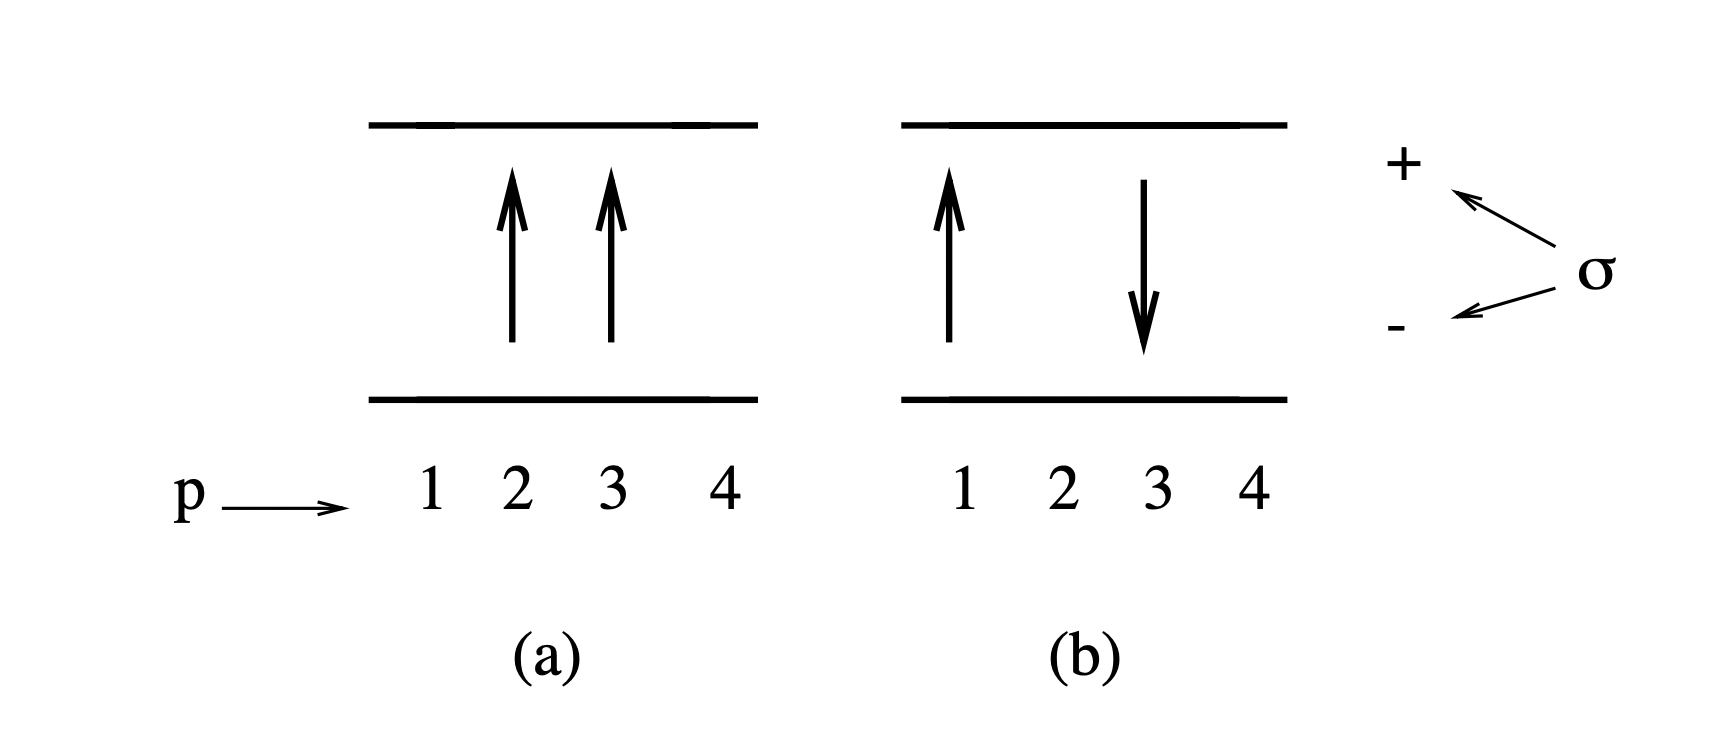
\includegraphics[width=.6\textwidth]{lipkin.png}
\end{figure}

It is a model which has been used widely in many-body physics and recently also in quantum computing, see for example
\url{https://journals.aps.org/prc/abstract/10.1103/PhysRevC.104.024305}.
In the weekly exercises (see week 37 and solutions) we showed that the quasispin operators

\[
\begin{array}{ll}
\hat{J}_{+}=&\sum_{p} a_{p+}^{\dagger}a_{p-}\\
&\\
\hat{J}_{-}=&\sum_{p}a_{p-}^{\dagger}a_{p+}\\
&\\
\hat{J}_{z}=&\frac{1}{2}\sum_{p\sigma}\sigma a_{p\sigma}^{\dagger}a_{p\sigma}\\
&\\
\hat{J}^{2}=&J_{+}J_{-}+J_{z}^{2}-J_{z}\\
&\\
\end{array}
\]
obey the commutation relations for angular momentum and that we could
express $\hat{H}$ in terms of the above quasispin operators and the number operator
\[
\hat{N}=\sum_{p\sigma}
a_{p\sigma}^{\dagger}a_{p\sigma}.
\]

\section{Problems} 
\subsection{Commutation relations (10pts)}
Show that $\hat{H}$ commutes with $J^{2}$, viz., $J$ is a good quantum number. Does it commute with $J_z$?

\subsection{Wick's theorem (10pts)}
Consider thereafter a state with all four fermions in the lowest level (see the above figure).
We can write this state as
\[
\ket{\Phi_0}=\ket{\Phi_{J_z=-2}} =a_{1-}^{\dagger}a_{2-}^{\dagger}
a_{3-}^{\dagger}a_{4-}^{\dagger}\ket{0}.
\]

This state has $J_{z}=-2$ (convince yourself that this is the case) and belongs
to the set of possible projections of $J=2$.  We introduce the
shorthand notation $\ket{J,J_z}$ for states with different values of
spin $J$ and its projection $J_z$.  We can think of this as our
computational basis for $J=2$ and all five projections $J_z$.  We will
also assume that the state $\Phi_0$ can be considered as an ansatz for
the ground state of the system. 

State Wick's time-independent theorem and use it to calculate the expectation values of
\[
\bra{\Phi_0}\hat{N}\ket{\Phi_0},
\]
and
\[
\bra{\Phi_0}\hat{H}\ket{\Phi_0}.
\]

For the expectation value of the energy (last equation), set up the relevant Feynman diagrams as well.




\subsection{Using quasispin operators (10pts)}
Show that you can obtain the same result for
\[
\bra{\Phi_0}\hat{H}\ket{\Phi_0}.
\]
using the quasispin representation of the Hamiltonian (plus the number operator). 
Comment your results.


\subsection{Setting up all basis states for $J=2$ (10pts)}

We will now use the quasispin operators to construct all possible states with spin $J=2$ using as starting point a state with all fermions in the lowest
single-particle state
\[
\ket{\Phi_{J_z=-2}} =a_{1-}^{\dagger}a_{2-}^{\dagger}
a_{3-}^{\dagger}a_{4-}^{\dagger}\ket{0}.
\]

This state has $J_{z}=-2$ and belongs to the set of projections for
$J=2$.  We will use the shorthand notation $\ket{J,J_z}$ for states
with different spon $J$ and spin projection $J_z$.  The other possible
states have $J_{z}=-1$, $J_{z}=0$, $J_{z}=1$ and $J_{z}=2$.

Use the raising or lowering operators $J_{+}$ and $J_{-}$  in order to construct the 
states for spin $J_{z}=-1$ $J_{z}=0$, $J_{z}=1$
and $J_{z}=2$.
The action of these two operators on a given state with spin $J$ and projection $J_z$
is given by ($\hbar = 1$) by
$J_+\ket{J,J_z}=\sqrt{J(J+1)-J_z(J_z+1)}\ket{J,J_z+1}$ and
$J_-\ket{J,J_z}=\sqrt{J(J+1)-J_z(J_z-1)}\ket{J,J_z-1}$.



\subsection{Finding the eigenvalues using Full Configuration Interaction Theory (10pts)}

Use the quasispin operators to construct the Hamiltonian matrix 
  $H$ for the five-dimensional space that has total spin $J=2$ and spin projections $J_z=-2,-1,0,1,2$.
Find thereafter the eigenvalues for the following parameter sets:
\[
\begin{array}{cccc}
(1)&\varepsilon=2,&V=-1/3,&W=-1/4\\
(2)&\varepsilon=2,&V=-4/3,&W=-1
\end{array}
\]
Which state do you expect to be the ground state?
Compute the eigenvalues by diagonalizing the Hamiltonian matrix and 
comment your results in terms of the coefficients of the various eigenfunctions and the parameters of the two Hamiltonians (1) and (2). 



\subsection{Hartree-Fock theory, general part (10pts)}
The standard way to perform a Hartree-Fock calculation is to
expand the single-particle functions in a known basis  and vary the coefficients,  that is, the new function single-particle wave function $|p\rangle$ is written as a linear expansion in terms of a fixed basis $\phi$
\begin{equation*} 
\psi_p  = \sum_{\lambda} C_{p\lambda}\phi_{\lambda},
\end{equation*}

This lead to a new Slater determinant which is related to the
previous via a unitary transformation.  
We consider a Slater determinant built up of single-particle orbitals
$\phi_{\lambda}$ where the indices $\lambda$ refer to specific
single-particle states. 

The unitary transformation

\begin{equation*}
\psi_p  = \sum_{\lambda} C_{p\lambda}\phi_{\lambda},
\end{equation*}
brings us into the new basis $\psi$.  The new basis is orthonormal and $C$ is a unitary matrix.


Minimizing with respect to $C^*_{p\alpha}$, remembering that
$C^*_{p\alpha}$ and $C_{p\alpha}$ (and that the indices contain all
single-particle quantum numbers including spin) are independent and
defining

\begin{equation*}
h_{\alpha\gamma}^{HF}=\langle \alpha | h | \gamma \rangle+
\sum_{p}\sum_{\beta\delta} C^*_{p\beta}C_{p\delta}\langle \alpha\beta|V|\gamma\delta\rangle_{AS},
\end{equation*}
show that you can write the Hartree-Fock  equations as

\begin{equation*}
\sum_{\gamma}h_{\alpha\gamma}^{HF}C_{p\gamma}=\epsilon_p^{\mathrm{HF}}C_{p\alpha}.
\label{eq:newhf}
\end{equation*}

Explain the meaning of the different terms and define the Hartree-Fock
operator in second quantization. Write down its diagrammatic
representation as well.  The greek letters refer to the wave functions
in the original basis 
while roman letters refer to the new basis.


\subsection{Hartree-Fock theory for the Lipkin model (10pts)}

The single-particle states for the Lipkin model
\[
\ket{u_{\sigma =-1,p}}=a_{-p}^{\dagger}\ket{0}
\hspace{1cm}
\ket{u_{\sigma =1,p}}=a_{+p}^{\dagger}\ket{0}
\]
can now be used as basis for a new single-particle state
$\ket{\phi_{\alpha ,p}}$  via a unitary  transformation
\[
\ket{\phi_{\alpha ,p}}=
\sum_{\sigma =\pm1}C_{\alpha\sigma}\ket{u_{\sigma ,p}}
\]
with $\alpha=\pm 1$ and $p=1,2,3,4$. Why is $p$ the same in 
$\ket{\phi}$
as in $\ket{u}$?  Show that the new basis is orthonormal given that the old basis is orthonormal.
Show that the new Slater determinant constructed from the new single-particle wave functions can be
written as the determinant based on the previous basis and the determinant of the matrix $C$.
Show that the old and the new Slater determinants are equal up to a complex constant with absolute value unity.
(Hint, $C$ is a unitary matrix).  Show also that the Slater determinants are orthogonal if we employ a single-particle basis which is orthogonal.



\subsection{Hartree-Fock energy (15pts)}

With the new basis we can construct a new Slater determinant given by
$\ket{\Psi}$
\[
\ket{\Psi}=\prod_{p=1}^{4}b_{\alpha ,p}^{\dagger}\ket{0}
\]
with $b_{\alpha ,p}^{\dagger}\ket{0}=\ket{\phi_{\alpha ,p}}$.
Use the Slater determinant from the previous exercise to calculate
\[
E=\bra{\Psi}H\ket{\Psi},
\]
as a function of the coefficients $C_{\sigma\alpha}$. We assume the coefficients are real.

\subsection{Stability of the Hartree-Fock equations (15pts)}

Using our Hartree-Fock results for the energy, show that
\[
  \frac{\epsilon}{3} > V+W,
\]
has to be fulfilled in order to find a minimum in the energy. Comment your results.

Hint: calculate the functional derivative  of the energy with respect to the coefficients $C_{\sigma\alpha}$. 

Calculate the Hartree-Fock ground state energies for the same parameters you used to diagonalize the Hamiltonian matrix in part E, that is 
\[
\begin{array}{cccc}
(1)&\varepsilon=2,&V=-1/3,&W=-1/4\\
(2)&\varepsilon=2,&V=-4/3,&W=-1
\end{array}
\]
Comment the results. 

\end{document}

